\documentclass[final]{article}

% Compile with pdfLaTeX
\usepackage[a4paper,portrait,margin=7mm]{geometry}
\usepackage[T1]{fontenc}
\usepackage[utf8]{inputenc}
\usepackage{lmodern}
\usepackage{microtype}
\usepackage{graphicx}
\usepackage{xcolor}
\usepackage{tikz}
\usetikzlibrary{arrows.meta,positioning,fit,calc,shapes.geometric}
\usepackage[most]{tcolorbox}
\usepackage{enumitem}
\usepackage{multicol}
\usepackage{tabularx}
\usepackage{ragged2e}
\usepackage{titlesec}
\usepackage{parskip}
\usepackage{hyperref}

\pagestyle{empty}
\setlength{\parindent}{0pt}
\setlength{\parskip}{2pt}
\setlist[itemize]{leftmargin=1.15em,itemsep=0.15em,topsep=0.15em}
\renewcommand{\familydefault}{\sfdefault}

% ---------- Colours ----------
\definecolor{KIWiNavy}{HTML}{123653}
\definecolor{KIWiDark}{HTML}{0B2B49}
\definecolor{KIWiOrange}{HTML}{F28C28}
\definecolor{KIWiPale}{HTML}{F3F7FA}
\definecolor{KIWiBluePale}{HTML}{EAF3F8}
\definecolor{KIWiLine}{HTML}{D7E3EC}
\definecolor{KIWiText}{HTML}{182A3A}
\definecolor{KIWiGrey}{HTML}{526575}

% ---------- Section heading and content panels ----------
\newtcolorbox{sectionbox}[1]{
  enhanced,
  colback=white,
  colframe=KIWiLine,
  boxrule=0.8pt,
  arc=2.5mm,
  left=3mm,right=3mm,top=2mm,bottom=2mm,
  title={#1},
  colbacktitle=KIWiNavy,
  coltitle=white,
  fonttitle=\bfseries\normalsize,
  attach boxed title to top left={yshift=-1mm,xshift=0mm},
  boxed title style={
    colback=KIWiNavy,
    colframe=KIWiNavy,
    arc=2mm,
    left=3mm,right=3mm,top=1mm,bottom=1mm
  },
  before skip=3mm,
  after skip=1mm
}

\newcommand{\methoditem}[1]{%
  \textcolor{KIWiOrange}{\large\textbullet}\hspace{2mm}%
  \textbf{\color{KIWiDark}#1}\\[-1mm]
  \ignorespaces
}

\newcommand{\smalltag}[1]{%
  \tcbox[colback=KIWiBluePale,colframe=KIWiLine,arc=1mm,
  boxrule=0.5pt,left=2mm,right=2mm,top=0.8mm,bottom=0.8mm]{\small\textcolor{KIWiNavy}{#1}}%
}

% ---------- Architecture diagram styles ----------
\tikzset{
  archbox/.style={
    draw=KIWiLine, line width=0.9pt, rounded corners=2mm,
    fill=KIWiBluePale, align=center, text=KIWiDark,
    minimum height=19mm, text width=27mm, inner sep=2.5mm,
    font=\small
  },
  archboxorange/.style={
    archbox, draw=KIWiOrange, fill=orange!10
  },
  archarrow/.style={-{Latex[length=3mm]},draw=KIWiNavy,line width=1.2pt},
  archlabel/.style={font=\bfseries\small,text=KIWiDark}
}

\begin{document}
\fontsize{8.5}{10.5}\selectfont
\noindent\begin{minipage}[t][\dimexpr\textheight-10pt\relax][s]{\textwidth}
\color{KIWiText}

% ===================== HEADER =====================
\begin{minipage}[c]{0.20\textwidth}
  {\fontsize{22}{24}\selectfont\bfseries\color{KIWiOrange} thws}\\[1mm]
  {\fontsize{6}{7}\selectfont\color{KIWiDark}Technical University of\\Applied Sciences\\Würzburg-Schweinfurt}
\end{minipage}
\hfill
\begin{minipage}[c]{0.77\textwidth}
  \centering
  {\fontsize{23}{26}\selectfont\bfseries\color{KIWiDark} KIWi -- KI-Wissensassistenz}\\[2mm]
  {\fontsize{11}{14}\selectfont\bfseries\color{KIWiNavy}
  AI-Powered Knowledge Assistance for the THWS CampusPortal}\\[2mm]
  {\fontsize{7}{9}\selectfont\color{KIWiGrey}
  Retrieval-Augmented Generation (RAG)
  \quad\textbar\quad Local LLM
  \quad\textbar\quad University Knowledge Retrieval}
\end{minipage}

\vspace{1mm}
{\color{KIWiOrange}\rule{\textwidth}{2.2pt}}

% ===================== PROBLEM + OBJECTIVES =====================
\vspace{2mm}
\begin{minipage}[t]{0.485\textwidth}\vspace{0pt}
\begin{sectionbox}{Problem}
\begin{itemize}
  \item University information is distributed across different sources
  (e.g., CampusPortal, wikis and manuals).
  \item Finding relevant and up-to-date answers is time-consuming.
  \item Traditional search can struggle with natural-language questions
  and process-related context.
  \item University information requires privacy-conscious processing.
\end{itemize}
\end{sectionbox}
\end{minipage}
\hfill
\begin{minipage}[t]{0.485\textwidth}\vspace{0pt}
\begin{sectionbox}{Objectives}
\begin{itemize}
  \item Enable natural-language question answering about university processes.
  \item Retrieve relevant information from approved knowledge sources.
  \item Generate context-aware answers using RAG.
  \item Provide transparent answers with supporting source references and URLs.
  \item Support a locally hosted solution without external LLM APIs.
  \item Evaluate retrieval quality, answer correctness and response time.
\end{itemize}
\end{sectionbox}
\end{minipage}

\vfill
% ===================== METHODOLOGY =====================
\begin{sectionbox}{Methodology}
\begin{minipage}[t]{0.485\textwidth}\vspace{0pt}
  \methoditem{Data Ingestion}
  Available university knowledge records are collected from CSV files,
  combining synthetic data and publicly available THWS information.

  \methoditem{Data Preprocessing}
  Questions, answers, key facts, evidence and source details are cleaned
  and prepared for further processing.

  \methoditem{Text Chunking}
  Longer records are divided into smaller text passages while preserving
  relevant metadata and source information.
\end{minipage}
\hfill
\begin{minipage}[t]{0.485\textwidth}\vspace{0pt}
  \methoditem{Embedding Generation}
  BGE-M3 converts the text passages into numerical vector representations
  for semantic search.

  \methoditem{Information Retrieval}
  ChromaDB stores the embeddings and retrieves relevant passages based on
  the user's natural-language query.

  \methoditem{Answer Generation}
  Qwen 2.5 7B Instruct, running locally through Ollama, generates
  context-aware answers using retrieved information and provides
  supporting source references.
\end{minipage}
\end{sectionbox}

\vfill
% ===================== ARCHITECTURE =====================
\begin{sectionbox}{Architecture}
\centering
\vspace{2mm}
\resizebox{\linewidth}{!}{%
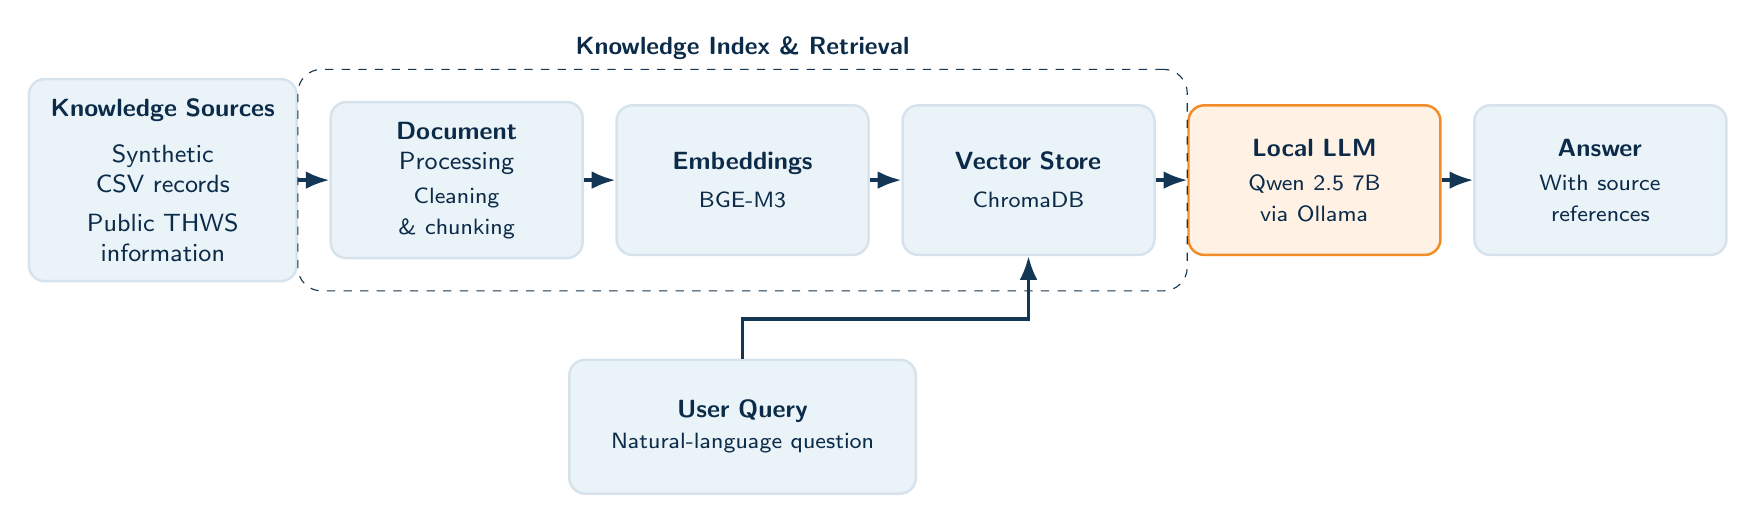
\begin{tikzpicture}[node distance=5mm and 4mm]

% Knowledge source
\node[archbox, text width=29mm, minimum height=25mm] (source) {
  \textbf{Knowledge Sources}\\[2mm]
  Synthetic CSV records\\[1mm]
  Public THWS information
};

\node[archbox, right=of source] (prep) {
  \textbf{Document}\\
  Processing\\[1mm]
  \footnotesize Cleaning\\\& chunking
};

\node[archbox, right=of prep] (embed) {
  \textbf{Embeddings}\\[1mm]
  \footnotesize BGE-M3
};

\node[archbox, right=of embed] (db) {
  \textbf{Vector Store}\\[1mm]
  \footnotesize ChromaDB
};

\node[archboxorange, right=of db] (llm) {
  \textbf{Local LLM}\\[1mm]
  \footnotesize Qwen 2.5 7B\\via Ollama
};

\node[archbox, right=of llm] (answer) {
  \textbf{Answer}\\[1mm]
  \footnotesize With source\\references
};

\draw[archarrow] (source) -- (prep);
\draw[archarrow] (prep) -- (embed);
\draw[archarrow] (embed) -- (db);
\draw[archarrow] (db) -- (llm);
\draw[archarrow] (llm) -- (answer);

% Query path
\node[archbox, below=13mm of embed, text width=39mm, minimum height=17mm] (query) {
  \textbf{User Query}\\
  \footnotesize Natural-language question
};

\draw[archarrow] (query.north) -- ++(0,5mm) -| (db.south);

% Dashed grouping for ingestion / retrieval components
\node[draw=KIWiNavy,dashed,rounded corners=3mm,inner sep=4mm,
fit=(prep)(embed)(db),
label={[archlabel]above:Knowledge Index \& Retrieval}] (retrievalgroup) {};

\end{tikzpicture}}
\vspace{3mm}

\footnotesize
\textcolor{KIWiGrey}{Knowledge ingestion prepares and indexes documents; at query time, relevant passages are retrieved and supplied to the local language model.}
\end{sectionbox}

\vfill
% ===================== DELIVERABLES / OUTCOMES =====================
\begin{sectionbox}{Deliverables / Expected Outcomes}
\begin{minipage}[t]{0.485\textwidth}\vspace{0pt}
  \begin{tcolorbox}[
    colback=orange!8,colframe=orange!35,arc=2mm,boxrule=0.6pt,
    title=\textbf{\color{KIWiDark}Deliverables},
    coltitle=KIWiDark,colbacktitle=orange!18]
    \begin{itemize}
      \item Working local RAG prototype.
      \item Automated CSV knowledge-ingestion pipeline.
      \item Persistent ChromaDB vector database.
      \item Terminal-based question-answering system.
      \item Source-supported answer generation.
    \end{itemize}
  \end{tcolorbox}
\end{minipage}
\hfill
\begin{minipage}[t]{0.485\textwidth}\vspace{0pt}
  \begin{tcolorbox}[
    colback=KIWiBluePale,colframe=KIWiLine,arc=2mm,boxrule=0.6pt,
    title=\textbf{\color{KIWiDark}Expected Outcomes},
    coltitle=KIWiDark,colbacktitle=KIWiLine]
    \begin{itemize}
      \item Faster access to university information.
      \item More transparent and evidence-grounded answers.
      \item Reduced reliance on external AI services.
      \item A foundation for future CampusPortal integration
      and a web-based interface.
    \end{itemize}
  \end{tcolorbox}
\end{minipage}
\end{sectionbox}

\vfill
% ===================== FOOTER =====================
\vspace{3mm}
\begin{tcolorbox}[
  colback=KIWiNavy,colframe=KIWiNavy,arc=2mm,
  boxrule=0pt,left=3mm,right=3mm,top=2mm,bottom=2mm]
\color{white}\fontsize{7}{9}\selectfont
\begin{tabularx}{\linewidth}{>{\centering\arraybackslash}X
                              >{\centering\arraybackslash}X
                              >{\centering\arraybackslash}X}
  \shortstack{\textbf{Team Members}\\{[Add team names]}}
  &
  \shortstack{\textbf{Supervisor}\\Prof. Dr. Ivan P. Yamshchikov}
  &
  \shortstack{\textbf{MAI Project}\\WS 2026/27}
\end{tabularx}
\end{tcolorbox}

\end{minipage}
\end{document}
